\documentclass[oneside]{Tptesi}
\usepackage[]{babel}
\usepackage[T1]{fontenc} % Usa la nuova codifica standard dei caratteri in LaTeX
\usepackage{graphicx}
\usepackage{rotating}
\usepackage{minted}
\usepackage{eurosym}
\usepackage{float}
\usepackage{hyperref}
\usepackage{amsfonts}
\usepackage{amsmath}
\newcommand\Chapter[2]{
  \chapter[#1: {#2}]{#1\\[2ex]\Large#2}
}
\newminted{rb}{baselinestretch=auto,tabsize=4,fontsize=\footnotesize,frame=lines,samepage=true}
\usepackage{pifont}
\usepackage{epstopdf}
\usepackage[italian]{varioref}
\usepackage[utf8]{inputenc}
\usepackage{graphicx}
\usepackage[export]{adjustbox}[2011/08/13]
\usepackage{caption}
\usepackage{subcaption}
\usepackage{booktabs} 
\usepackage{multirow}
\usepackage{url}
\hypersetup{urlcolor=black}
\usepackage{imakeidx}
\makeindex[title=Ciao]
				
% ------------------------------------------------------------------------------
% Metadata (Change this)
% ------------------------------------------------------------------------------
	\title{Disparity coherent stereo video watermarking}
	\author{Benedetta Barbetti, Michaela Servi}
	\titolocorso{Computer Engineering}
	\chair{Prof. Alessandro Piva}
	\numberofmembers{1} %numero dei relatori
	\othermembers{Prof. Paolo Nesi}
	\degreeyear{2014/2015}
	\numerocorrelatori{2} %numero dei correlatori
	\correlatori{Prof. Carlo Colombo\\ Dott. Pasquale Ferrara} 
	\dataTesi{December 2015}



% ---- Inclusioni separate da virgole e senza spazi  --------------
\includeonly 
{abstract, introduction, stereo_video, stereo_wat, spat_wat, freq_wat, conclusions, bibliografia}
%
%%//// document ///////////////////////////////////////////////////////////////

\begin{document}
\hyphenation{}
%
%
\maketitle % crea il frontespizio(ricordati di copiare "stemma.eps" nella tuadirectory)%

\thispagestyle{empty}
\begin{flushright}
\large\em \vspace*{2cm}

   
\end{flushright}

%----- Abstract
\begin{abstract}
Nowdays stereoscopic videos play an important role in many applications: from medical diagnosis and endoscopic surgery to fault detection in manufactory industry, army and arts, in people tracking and mobile robotics navigation as, naturally, in the film industry with 3D movie release.\\
The huge increase of distribution systems of this content leads to the increase of concerns over content copyright protection: in this thesis a blind disparity-coherent watermarking technique has been presented to protect stereoscopic video contents.\\
The algorithm belongs to view-based methods and operates in both frequency and spatial domain in a diparity-coherent way, namely, a physical point of the captured scene always carries the same watermark sample regardless of where it appears in the left and right views.\\
This kind of techniques has been proved to yield less visual discomfort and to be robust against view synthesis attacks, as shown by the experiments conducted on the implemented algorithm.


\end{abstract}
% --- Crea la pagina dei ringraziamenti (se ti va) ---

%% --- Fine ringraziamenti ----------------
%%
\pagenumbering{arabic}
\pagestyle{plain}
\tableofcontents % inserisce indice generale
\listoffigures   % inserisce indice figure
\listoftables    % inserisce indice tabelle
%\listoflistings	 % inserisce indice di codici
%%
%%--------------- Inizio del testo vero e proprio
%%

\cleardoublepage
\pagenumbering{arabic}
\pagestyle{headings}

%% ////////////////////////////////////////////////////////////////////////////
\chapter*{Introduction}
\markright{Introduction}
\label{intro}
\phantomsection
\addcontentsline{toc}{chapter}{Introduction}

In the last few years the stereoscopic technique has become a great part of image and video processing.\\
In medical diagnosis and endoscopic surgery as in fault detection in manufactory industry, army and arts,
multiview imaging is considered as a key enabler  for professional added value services.\\
Nowdays stereoscopic techniques are also used in people tracking and mobile robotics
navigation for economic reasons and to improve performances.\\
Finally the worldwide success of 3D movie releases and 3D video games and the deployment of 3D televisions made the nonprofessional user aware about a new type of multimedia entertainment experience.\\
The increasing production and distribution of these contents leads to the concerns over copyright protection.\\
Digital watermarking can be considered as the most flexible property right protection technology, since it adds some information (a mark, i.e. copyright information) in the
original content without altering its visual quality so that such a marked content can be further distributed/consumed by another user without any restriction; still, the legitimate/illegitimate usage can be determined at any moment by detecting the mark. In same case the watermarking protection mechanism, instead of restricting the media copy/distribution/consumption, provides means for tracking the source of the content illegitimate usage.\\
The purpose of this thesis is to provide a new watermarking system for copyright protection of stereoscopic videos. The method operates in the frequency and in the spatial domain by embedding a pseudo-random sequence of real numbers in a selected set of DFT coefficients of the left image; then the reference watermark is distorted according to the depth information prior to insertion and spatially added to the right image.\\
In Chapter \ref{}...
\chapter{Stereoscopic Video}
\markright{Stereoscopic Video}
\label{stereo_video}
\phantomsection
%\addcontentsline{toc}{chapter}{Stereoscopic Video}

In a wide variety of image processing applications, explicit depth information is required in
addition to general image informations, such as intensities, color, densities.\\
Examples of such applications are found in 3D vision (robot vision, photogrammetry, remote sensing systems), in medical imaging (computer tomography,
magnetic resonance imaging, microsurgery), in remote handling of objects (random bin picking), in space exploration (mobile robotics navigation) or 3D movies and videogames.\\
In each of these cases, depth information is essential for accurate image analysis or for enhancing the
realism.\\
In remote sensing the terrain's elevation needs to be accurately determined for map production, in remote handling an operator needs to have precise knowledge of the threedimensional organization of the area to avoid collisions and misplacements.\\
\begin{figure}[h!]
\centering
\begin{subfigure}[]{0.5\textwidth}
		\centering
        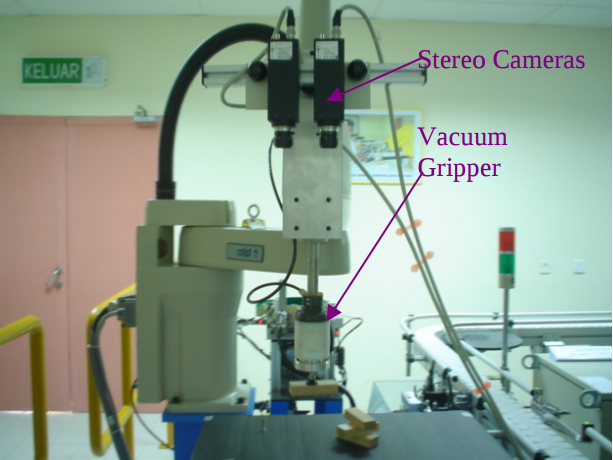
\includegraphics[width=0.7\textwidth]{./img/bin_pick.png}
                \caption{\scriptsize{In bin picking applications stereo vision helps to reconstruct the 3D environment and detect the part of the object to be robotically picked}}
\end{subfigure}% 
~ \quad
\begin{subfigure}[]{0.5\textwidth}
	\centering
	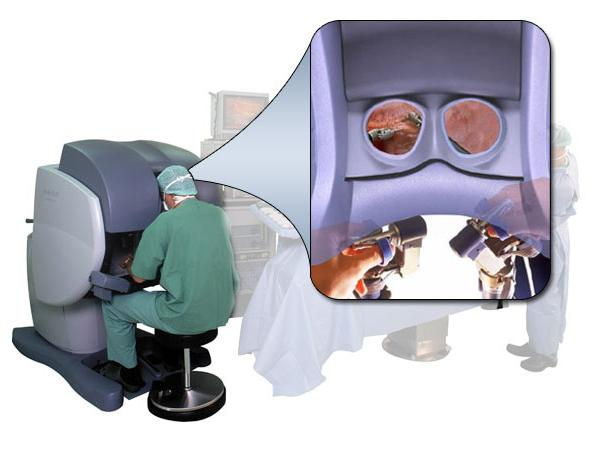
\includegraphics[width=0.7\textwidth]{./img/da_vinci.jpg}
          \caption{\scriptsize{Surgical robot \textit{Da vinci} is provided with a stereoscopic camera that allows a tridimensional view of the operative filed.}}
\end{subfigure} 
\caption{\small{Stereoscopy in medical and industrial field}}
\end{figure}

\begin{figure}[h!]
\centering
\begin{subfigure}[]{0.5\textwidth}
		\centering
        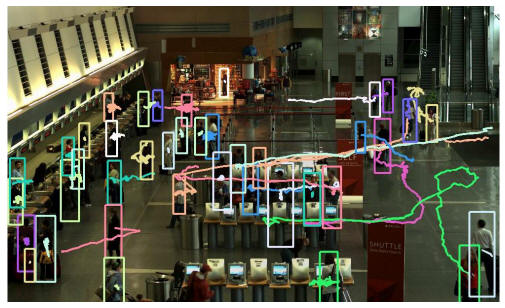
\includegraphics[width=0.7\textwidth]{./img/tracking.jpg}
                \caption{\scriptsize{In people tracking application stereo vision improves segmentation thanks to depth information and it's less sensible to light changes.}}
\end{subfigure}% 
~ \quad
\begin{subfigure}[]{0.5\textwidth}
		\centering
        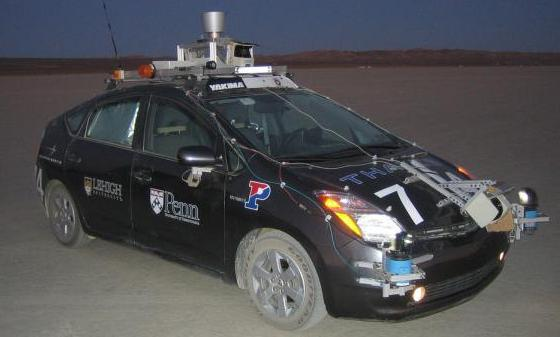
\includegraphics[width=0.7\textwidth]{./img/little_ben.jpg}
                \caption{\scriptsize{In mobile robotics navigation stereo vision has became the first choice technology because it provids a lot of quality data for low costs.}}
\end{subfigure} 
\caption{\small{Stereoscopy application's fields}}
\end{figure}
Depth in real world scenes can be explicitly measured by a number of range sensing devices such as by laser range sensors, by structured light or by ultrasound.
However it's usually undesirable to have separate systems for acquiring the intensity and the depth
information because of the relative low resolution of the range sensing devices and because it's not an easy task to fuse information from different type of sensors; for these reasons and for a non-negligible economic factor stereoscopic vision has becoming the technology of choice in these type of applications.
\begin{figure}[h!]
\centering
\begin{subfigure}[]{0.4\textwidth}
		\centering
        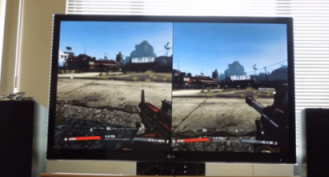
\includegraphics[width=0.7\textwidth]{./img/games1.png}
                \caption{\scriptsize{Stereo video frames, left and right.\newline}}
\end{subfigure}
\begin{subfigure}[]{0.4\textwidth}
		\centering
        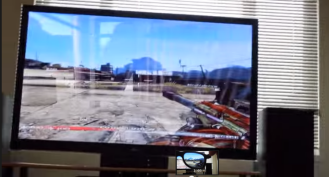
\includegraphics[width=0.7\textwidth]{./img/games2.png}
                \caption{\scriptsize{Overlap of the two frames.}}
\end{subfigure} 
\begin{subfigure}[]{0.4\textwidth}
		\centering
        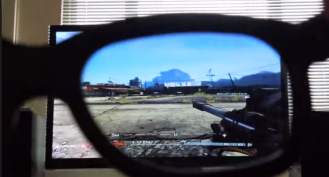
\includegraphics[width=0.7\textwidth]{./img/games3.png}
                \caption{\scriptsize{3D view with specific glasses}}
\end{subfigure}%
\begin{subfigure}[]{0.4\textwidth}
		\centering
        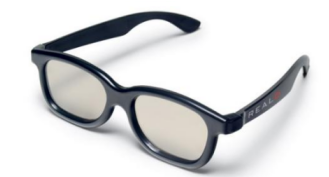
\includegraphics[width=0.7\textwidth]{./img/games4.png}
                \caption{\scriptsize{Polarized glasses for 3D view}}
\end{subfigure} 
\caption{\small{Stereoscopy in 3D video games}}
\end{figure}

\section{Stereo vision}
In image processing stereo vision is the process of extracting 3D information from multiple 2D views of a scene. \\
The 3D information can be obtained from a pair of images, also known as a stereo pair, by estimating the relative depth of points in the scene.\\
From the anatomic point of view, the human brain calculates the depth in a visual scene mainly by
processing the information brought by the images seen by the left and the right eyes. These left and right images are slightly different because the eyes have biologically different emplacements.\\
Consequently, the straightforward way of achieving stereoscopic digital imaging is to emulate the
Human Visual System (HSV) by setting-up (under controlled geometric positions), two traditional 2D
cameras.\\
\begin{figure}[h]
\centering
\begin{subfigure}[b]{0.35\textwidth}
        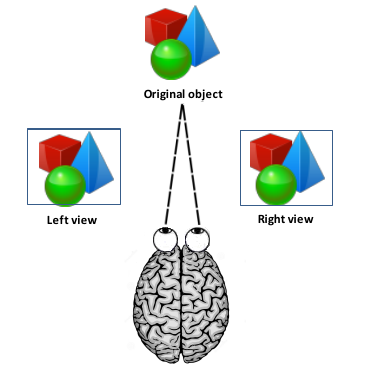
\includegraphics[width=\textwidth]{./img/hvs.png}
         \caption{\scriptsize{Binocular human visual system}}
         \label{fig:hvs}
\end{subfigure}
\begin{subfigure}[b]{0.35\textwidth}
        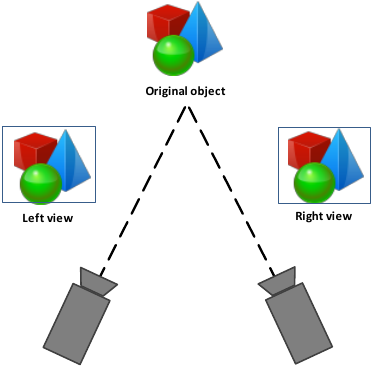
\includegraphics[width=\textwidth]{./img/stereo.png}
        \caption{\scriptsize{Stereoscopic system}}
        \label{fig:stereo}
\end{subfigure} 
\caption{\small{Binocular human vision vs. stereoscopic content acquisition.}}
\end{figure}

\subsection{Acquisition of stereoscopic images}\label{sec:acquisition-of-stereoscopic-images}

In order to be able to perceive depth using recorded images, a stereoscopic camera is required,
which consists of two cameras that capture two different, horizontally shifted perspective
viewpoints; with two (or more) cameras we can infer depth, by means of triangulation, if we are able to find corresponding points in the two images (Figure).\\
\begin{figure}[h!]
\centering
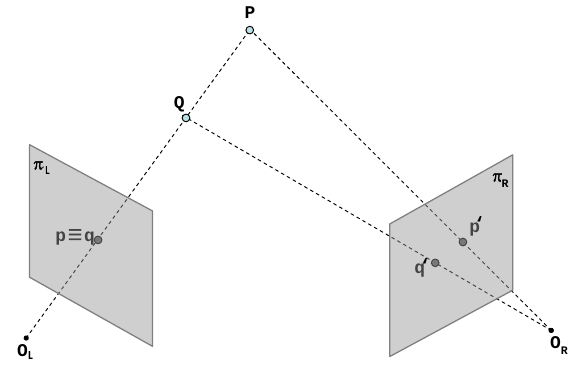
\includegraphics[width=0.6\textwidth]{./img/correspondance.png}
\caption{\small{Triangulation: with two cameras the depth of }}
\label{fig:corr}
\end{figure}
 The camera setup should be geometrically
calibrated such that the two cameras capture the same part of the real world scene.\\
Calibration of a stereo camera system involves the estimation of the intrinsic and extrinsic parameters of the model: intrinsic parameters embody the characteristics of the optical system and its geometric relationship with the image sensor, extrinsic parameters relate the location and orientation of the second camera with respect to the first one in the 3D space (Figure).\\
\begin{figure}[h!]
\centering
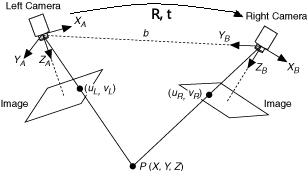
\includegraphics[width=0.6\textwidth]{./img/stereo_system.png}
\caption{\small{Stereo camera model}}
\label{fig:rt}
\end{figure}
These parameters can be used to rectify a stereo pair of images to make them appear as the two image planes are parallel (Figure); once the images are rectified, epipolar geometry it's used to find corresponding points and compute the disparity map.\\
\begin{figure}[h!]
\centering
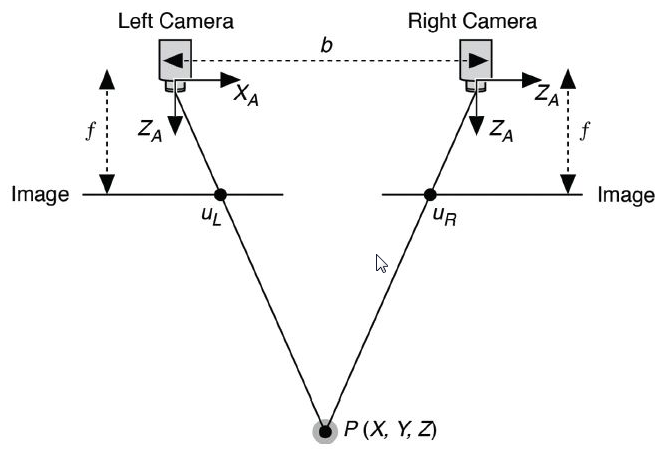
\includegraphics[width=0.6\textwidth]{./img/rect_stereo.png}
\caption{\small{Rectified stereo cameras}}
\label{fig:rect_stereo}
\end{figure}
\begin{figure}[h!]
\centering
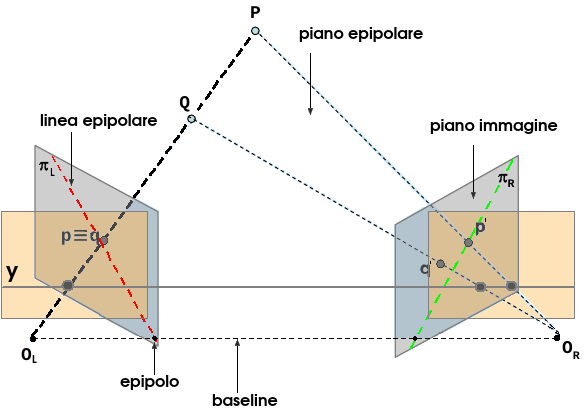
\includegraphics[width=0.6\textwidth]{./img/standard.png}
\caption{\small{Rectified images: corresponding points (p, p'), projection of the same 3D point (P) are constrained on the same image horizontal line, the epipolar line}}
\label{fig:std}
\end{figure}

\newpage
\subsection{Disparity map computation}

With the stereo rig in standard form and by considering similar triangles in Figure XX (PO$_{L}$O$_{R}$ and Ppp'): 
$$
\frac{b}{Z} = \frac{(b+x_{L}) - x_{R}}{Z-f} 
$$ 
so
$$
Z = \frac{b \cdot f}{x_{L} - x_{R}} = \frac{b \cdot f}{d}
$$ 

where $ d = x_{L} - x_{R} $ it's called \textit{disparity}.\\
\begin{figure}[h!]
\centering
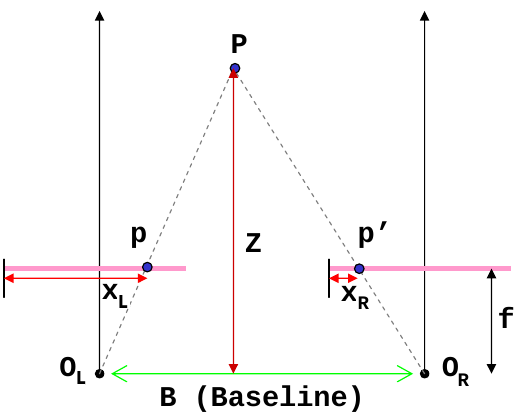
\includegraphics[width=0.6\textwidth]{./img/depth.png}
\caption{\small{Geometry of standard form}}
\label{fig:depth}
\end{figure}
Disparity is, therefore, the difference between the $x$ coordinates of two corresponding points and it is usually encoded with greyscale image (Figure XX), where points closer to the cameras are brighter and correspond to a higher disparity.\\
\begin{figure}[h!]
\centering
\begin{subfigure}[]{0.4\textwidth}
\centering
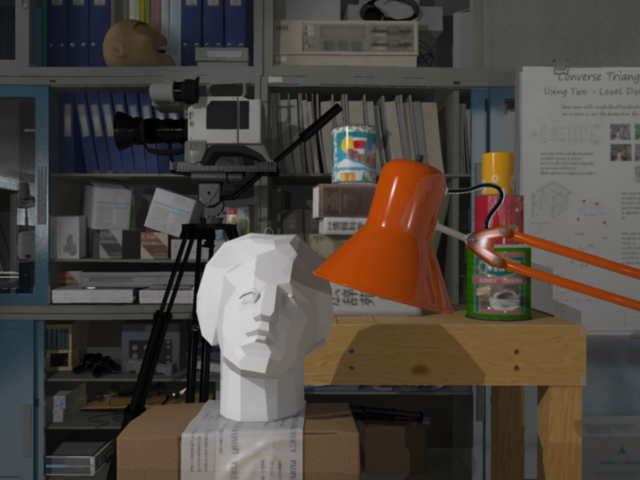
\includegraphics[width=0.7\textwidth]{./img/left.png}
\caption{\scriptsize{Left image}}
\end{subfigure}% 
~ %add desired spacing between images, e. g. ~, \quad, \qquad, \hfill etc.$  $
  %(or a blank line to force the subfigure onto a new line)
\begin{subfigure}[]{0.4\textwidth}
\centering
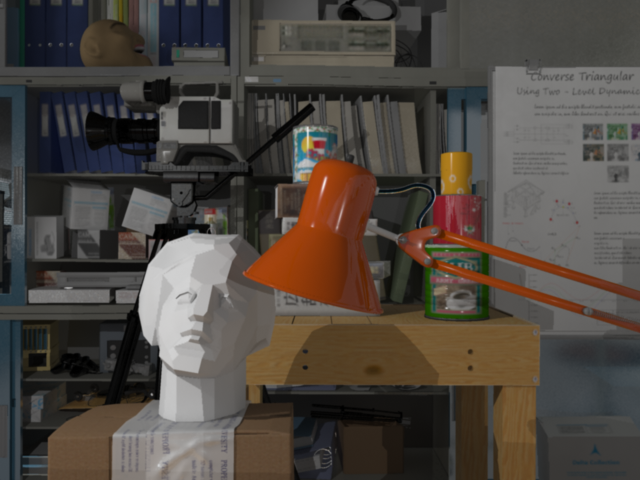
\includegraphics[width=0.7\textwidth]{./img/right.png}
\caption{\scriptsize{Right image}}
\end{subfigure} 
~\quad
\begin{subfigure}[]{0.4\textwidth}
\centering
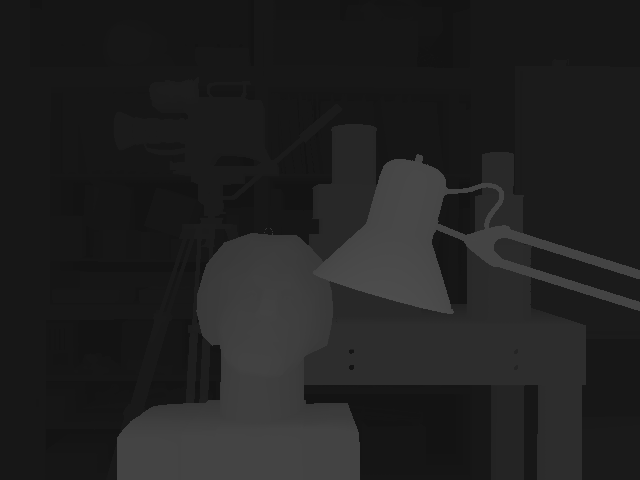
\includegraphics[width=0.7\textwidth]{./img/disparity.png}
\caption{\scriptsize{Disparity map}}
\label{disparity}
\end{subfigure}%
\caption{\small{Stereo pair and disparity map}}
\end{figure}
In order to compute the disparity map is necessary to find corresponding points; stereo correspondance is though a challenging task that has to manage with perspective distortions, uniform and ambiguous regions, repetitive patterns, occlusions and discontinuities(Figure XX).\\
\begin{figure}[h!]
\centering
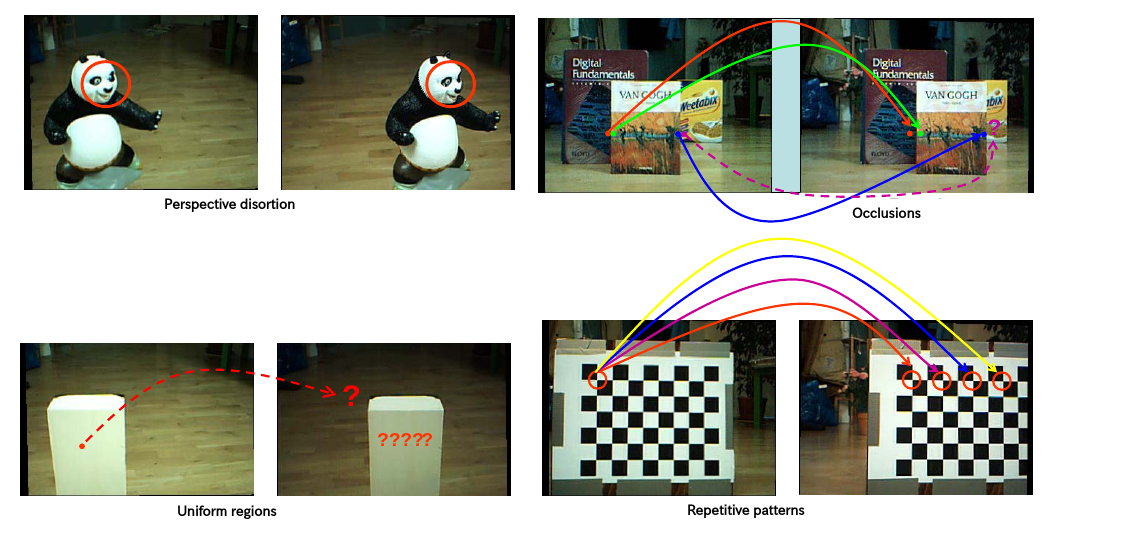
\includegraphics[width=0.6\textwidth]{./img/occl.png}
\caption{\small{Stereo matching general problems}}
\label{fig:occl}
\end{figure}
In general, stereo matching algorithms can be categorized into two major classes:
\begin{itemize}
\item local methods
\item global methods.
\end{itemize}
Local stereo algorithms estimate the correspondence using a local support region or a window. Local algorithms generally rely on an approximation of the smoothness constraint assuming that all pixels within the matching region have the same disparity. However, this assumption is not valid for highly curved surfaces or around disparity discontinuities.\\
A naive approach consists of comparing each  pixel or window in the left image with every pixel or window on the same epipolar line in right image and picking position with minimum match cost (e.g., SSD, SAD, normalized correlation).\\ 
\begin{figure}[h!]
\centering
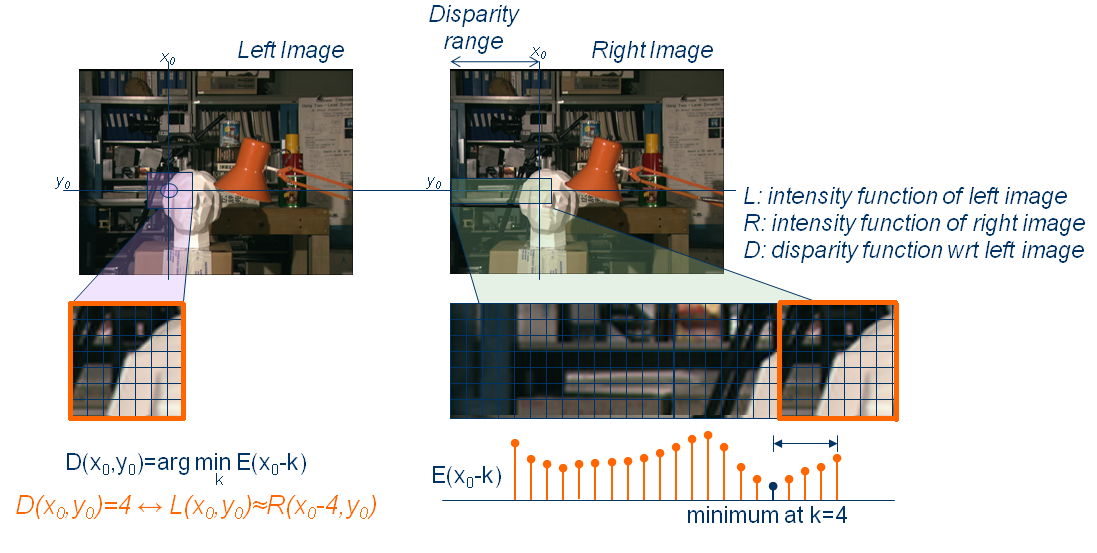
\includegraphics[width=0.7\textwidth]{./img/local.png}
\caption{\small{Local stereo matching, window based}}
\label{fig:local}
\end{figure}
Global stereo methods consider stereo matching as a labeling problem where the pixels of the reference image are nodes and the estimated disparities are labels. An energy functional embeds the matching assumptions by its data, smoothness, and occlusion terms and propagates them along the scan line or through the whole image. The labeling problem is solved by energy functional minimization, using dynamic programming, graph cuts, or belief propagation.\\
Even if this class of algorithms is significantly slow, the results, especially when textures and discontinuities are present, are much accurate.\\
\newline
In this thesis the Kolmogorov and Zabih's Graph Cuts Stereo Matching Algorithm has been used, because there were no time constraints requirements and the quality of the computed disparities has been considered satisfying regard to the ground trouth.\\








\section{Acquisition of stereo images}


\section{Display 3D video}

\chapter{Stereoscopic video watermarking: state of art}
\markright{Stereoscopic video watermarking: state of art}
\label{soa}
\phantomsection
%\addcontentsline{toc}{chapter}{Model with phase type approximation}
\section{State of art}
\chapter{Disparity-coherent watermarking in the spatial domain}
\markright{Disparity-coherent watermarking in the spatial domain}
\label{spat_wat}
\phantomsection
%\addcontentsline{toc}{chapter}{Prism Modelling}
\chapter{Disparity-coherent watermarking in the Fourier domain}
\markright{Disparity-coherent watermarking in the Fourier domain}
\label{freq_wat}
\phantomsection
%\addcontentsline{toc}{chapter}{Prism Model Rewards}

\chapter{Conclusions}
\markright{Conclusions}
\phantomsection
%\addcontentsline{toc}{chapter}{Conclusions}


\phantomsection
\addcontentsline{toc}{chapter}{Bibliografia}
\bibliographystyle{plain}
\bibliographystyle{plain}
\begin{thebibliography}{99}

\bibitem{MED} P.-L. Chang, D. Stoyanov, A. Davison, and P. E. Edwards, Real-time
dense stereo reconstruction using convex optimisation with a cost-volume for image-guided robotic surgery, Proc. MICCAI,2013

\bibitem{MED2}Bhayani SB, Andriole GL.,Three-Dimensional (3D) Vision: Does It Improve Laparoscopic Skills? An Assessment of a 3D Head-Mounted Visualization System. Reviews in Urology. 2005;7(4):211-214


\bibitem{TRACK}Muñoz-Salinas, Rafael, Eugenio Aguirre, and Miguel García-Silvente, People detection and tracking using stereo vision and color. Image and Vision Computing 25.6 (2007): 995-1007

\bibitem{PG} Point Grey Stereo Vision Introduction and Applications \url{http://www.ptgrey.com/support/downloads/10353}


\bibitem{GAME} \url{http://www.nvidia.com/docs/IO/66368/Top-10-3D-Games-by-APC.PDF}


\bibitem{BP} Radhakrishnamurthy, H.Ch. et al.: Stereo Vision System for A Bin Picking Adept Robot, Malaysian Journal of Computer Science. Vol. 20, No. 1, 2007, pp. 91 - 98 

\bibitem{DEVICE} A Beginner's Guide to Shooting Stereoscopic 3D \\ \url{http://www.dashwood3d.com/blog/beginners-guide-to-shooting-stereoscopic-3d/}

\bibitem{BUMBLE} \url{https://www.ptgrey.com//bumblebee2-firewire-stereo-vision-camera-systems}

\bibitem{AUTO}\url{http://www.autonomoustuff.com/stereo-vision.html}

\bibitem{SV}Stefano Mattoccia, Stereo Vision: Algorithms and Applications
\url{www.vision.deis.unibo.it/smatt}

\bibitem{SV2}P. K. Sinha, Image Acquisition and Preprocessing for Machine Vision Systems, SPIE Press, Bellingham (2012)

\bibitem{ZISS}Hartley, R. and Zisserman, A. 2000. Multiple view geometry in computer vision, Cambridge University Press: Cambridge, UK


\bibitem{KZ}Vladimir Kolmogorov, Pascal Monasse, and Pauline Tan, Kolmogorov and Zabih’s Graph Cuts Stereo Matching Algorithm, Image Processing On Line, 4 (2014), pp. 220–251. \url{http://dx.doi.org/10.5201/ipol.2014.97}

\bibitem{ALPHA}D. Batra, P. Kohli, Making the right moves: guiding alpha-expansion using local primal-dual gaps, in: IEEE Conference on Computer Vision and Pattern Recognition (CVPR), 2011

\bibitem{3D} \url{http://www.sky.com/shop/__PDF/3D/Basic_Principles_of_Stereoscopic_3D_v1.pdf}

\bibitem{3D2} \url{http://www.techradar.com/news/television/active-shutter-vs-passive-3d-tv-which-is-best-958717}

\bibitem{COX}Cox, Ingemar J., et al. "Secure spread spectrum watermarking for multimedia." Image Processing, IEEE Transactions on 6.12 (1997): 1673-1687

\bibitem{COX1}Cox I, Miller M, Bloom J (2002) Digital watermarking. Morgan Kaufmann, San Mateo


\bibitem{COX2} Cox I, Miller M, Bloom J (2002) Digital watermarking. Morgan Kaufmann, San Mateo

\bibitem{SH} Shannon CE (1958) Channel with side information at the transmitter. IBM Journal of Research and Development 2(4):289–293

\bibitem{EG} Eggers JJ, Bäuml R, Tzschoppe R, Girod B (2003) Scalar Costa scheme for information embedding. IEEE Trans Signal Process 51(4)

\bibitem{COSTA} Costa MHM (1983) Writing on dirty paper. IEEE Trans Inf Theory IT-29(3):439–441


\bibitem{16}Dong-Choon H, Kyung-Hoon B, Eun-Soo K (2003) Real-time stereo image watermarking using discrete cosine transform and adaptive disparity maps. Multimedia Systems Appl VI, Proc SPIE 5241:233

\bibitem{17}Dong-Choon H, Kyung-Hoon B, Eun-Soo K (2003) Stereo image watermarking scheme based-on discrete wavelet transform and adaptive disparity estimation. Mathematics of data/image coding, compression, and encryption, with applications. Conference no. 6, San Diego

\bibitem{18}Kumar S, Raman B, Thakur M (2009) Real coded genetic algorithm based stereo image watermarking. IJSDA Int J Secure Digit Inf Age 1(1)

\bibitem{19}Bhatnager G, kumar S, Raman B, Sukavanam N (2009) Stereo coding via digital watermarking. J Electron Imaging 18(3)

\bibitem{20}Campisi P (2008) Object-oriented stereo image digital watermarking. J Electron Imaging 17(4):043024

\bibitem{21}Yu M, Wang A, Luo T, Jiang G, Li F, Fu S (2011) New block relationship based stereo image watermarking algorithm. In: The sixth international conference on systems and networks communications, ICSNC 2011, pp 171–174 (October 2011)

\bibitem{22}Zhang Z, Zhu Z, Xi L (2007) Novel scheme for watermarking stereo video. Int J Nonlinear Sci 3(1):74–80

\bibitem{QIM}Hasnaoui M, Belhaj M, Mitrea M, Prêteux F (2011) mQIM principles for MPEG-4 AVC watermarking, SPIE Photonics West 2011 (January 2011)

\bibitem{QIM1}Belhaj M, Mitrea M, Duta S, and Preteux F (2010) MPEG-4 AVC robust video watermarking based on QIM and perceptual masking. In: International conference on communication, Bucharest (June 2010)

\bibitem{METRICS}Joshi, Madhuri A., et al. Image and Video Compression: Fundamentals, Techniques, and Applications. CRC Press, 2014

\bibitem{QMETRICS} Hewage, Chaminda TER, and Maria G.Martini, Edges-based reduced-reference quality metric for 3D video compression and transmission. Selected Topics in Signal Processing, IEEE Journal of 6.5 (2012): 471-482.



\bibitem{DOER}Faridul, Hasan Sheikh, Gwenaël Doërr, and Séverine Baudry, Disparity estimation and disparity-coherent watermarking. IST/SPIE Electronic Imaging. International Society for Optics and Photonics, 2015.


\bibitem{STAT}L. Scharf, Statistical Signal Processing: detection,
estimation, and time series analysis, Add. Wesley,
1991.






\end{thebibliography}
\clearpage
\thispagestyle{empty}
\end{document}